\section{Versuchsaufbau/-durchführung}

\subsection{Versuchsaufbau}

Der normale und anomale Zeemaneffekt soll mit Hilfe der roten (normaler Zeemaneffekt)
und der blauen (anomaler Zeemaneffekt) Spektralinie einer $\ce{Cd}$-Lampe untersucht werden.
Das für die Energieaufspaltung benötigte Magnetfeld wird von einem Elektromagnet erzeugt,
Deshalb wird die Lampe zwischen die Polschuhe des Elektromagneten gestellt.
Das von der Lampe ausgehende Licht wird in einem optischen Aufbau gebündelt und aufgespaltet
in eine Lummer-Gehrcke Platte geleitet. Der optische Aufbau und der grundlegende Versuchsaufbau
sind in Abbildung \ref{fig: versuchsaufbau} skizziert. Das Linsensystem dient zur Bündelung und Fokussierung des Lichtes und
mit dem Geradsichtprisma soll das Licht in seine Spektrallinien aufgespalten werden.
\FloatBarrier
\begin{figure}[h]
  \centering
  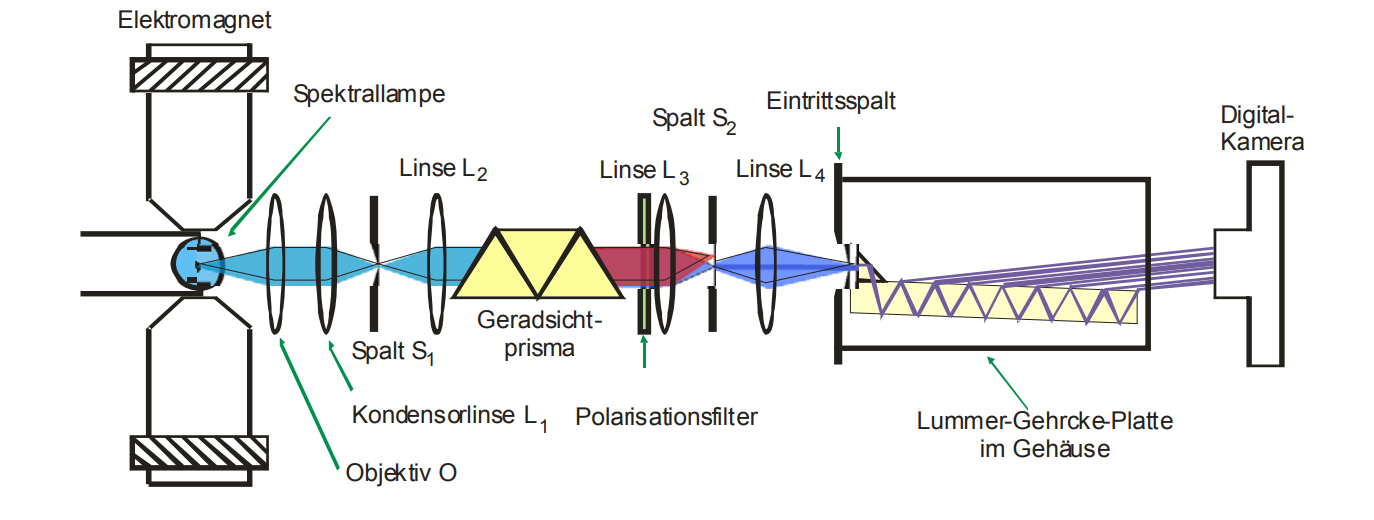
\includegraphics[width=0.85\textwidth]{pics/versuchsaufbau.png}
  \caption{Versuchsaufbau zur Untersuchung des Zeeman-Effektes \cite{anleitung27}.}
  \label{fig: versuchsaufbau}
\end{figure}
\FloatBarrier

Der in der Abbildundung \ref{fig: versuchsaufbau} zu sehende Polarisationsfilte wird dazu genutzt
die $\pi$ und $\sigma$ Übergänge zu unterscheiden. Das verwendent einer Lummer-Gehrcke Platte
bietet sich immer dann an, wenn ein besonders hohes Auflösungsvermögen benötigt wird
und nur monochromatisches Licht untersucht werden soll.
Das Auflösungsvermögen kann mittels
\begin{equation}
  \label{eq: auflösungsvermoegen_lummer}
  A=\frac{L}{\lambda}(n(\lambda)^2-1)
\end{equation}
berechnet werden, hierbei ist L die Länge der Platte, $\lambda$ die Wellenlänge
des zu untersuchenden Lichtes und $n(\lambda)$ der wellenlängenabhängige
Brechnungsindex der Platte. Mit Hilf eiens Primas wird licht in Platte eingeleitet.
Das Licht wird innerhalb der Platte fast vollständig reflektiert, der transmitierte
Teil interferiert. Damit es zu konstruktiver Interferenz kommt muss die Bragg-Bedingung
\begin{equation*}
  2d\cos(\theta)=n\lambda
\end{equation*}
erfüllt sein. Die in der Bragg-Bedingung auftretenden Größen sind die Dicke der Platte $d$,
die Wellenlänge $\lambda$ und die Ordnung des Maximas $n$.
Wird monochromatisches Licht in die Lummer-Gehrcke Platte eingestrahlt, ist der
Gangunterschied der Interferenzstreifen gleich der Wellenlänge $\lambda$.
Die Funktionsweise der Lummer-Gehrcke Platte ist in Abbildung \ref{fig: lummer} zu erkennen.
\FloatBarrier
\begin{figure}[h]
  \centering
  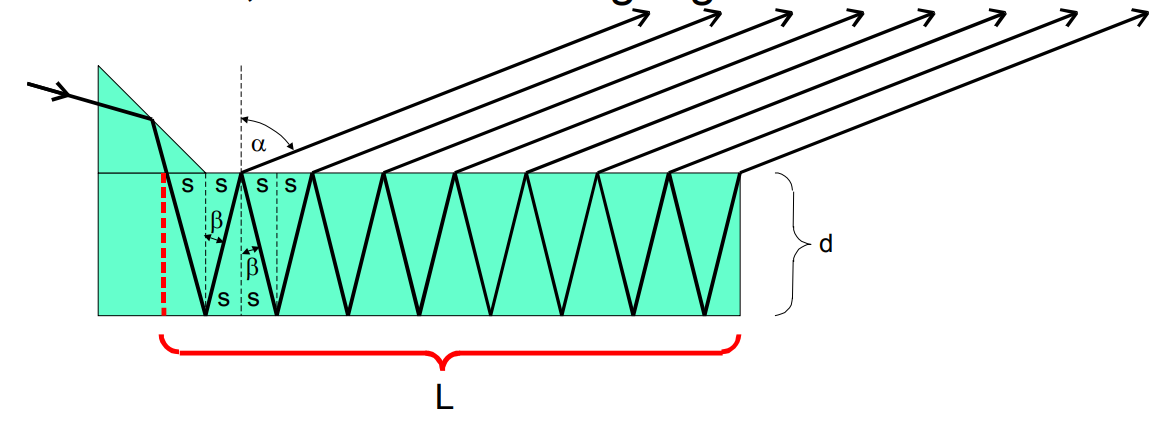
\includegraphics[width=0.7\textwidth]{pics/lummer.png}
  \caption{Aufbau einer Lummer-Gehrcke Platte \cite{anleitung27}.}
  \label{fig: lummer}
\end{figure}
\FloatBarrier
Zwei unterschiedliche Wellenlängen werden von einer Lummer-Gehrcke Platte bis zu
einer Längendifferenz von
\begin{equation}
  \label{eq: lummer_wellendif}
  \delta \lambda\ua{D}=\frac{\lambda^2}{2 d} \sqrt{\frac{1}{n^2-1}}
\end{equation}
unterscheidbar aufgelöst. Die Größe $\delta \lambda\ua{D}$ wird auch als Dispersionsgebiet
bezeichnet.

\subsubsection{Versuchsdurchführung}
Zu nächst muss die optische Apperatur so eingestellt werden das Licht mit einer hohen Helligkeit
an der Lummer-Gehrcke Platte ankommt. Die einzelen Spalte werden so angepasst das die
einzelnen Spektrallinien möglichst dünn und scharf sind.

Anschließend wird der Elektromagnet geeicht und auf Hystereseeffekte untersucht.
Dazu wird mittels einer Hall-Sonde die Magnetfeldstärke für Stromstärken
zwischen $\num{1}-\num{20}\,\si{\ampere}$ gemessen. Um gleichzeitig den Magnet auf Hysteresseeffekte zu untersuchen,
wird die Magnetfeldstärke auf einem aufsteigenden Ast ($I_i>I_j,\, i>j$) untersucht und einmal auf einem absteigenden ($I_i<I_j,\, i>j$).

Als erstes wird rotes Licht $\lambda = \SI{643.8}{\nano\meter}$ untersucht \cite{anleitung27}.
Licht dieser Wellenlänge wird beim Übergang $^1P_1\leftrightarrow ^1\!\!D_2$ emitiert \cite{anleitung27}.
Für eine optimale Untersuchung muss die Digitalkamera so ausgerichtet werden, dass sie $10-12$ Maxima aufnimmt.
Ist die Kamera richtig justiert so wird ein Foto von dem Interferenzbild ohne Magnetfeld gemacht, eine beispielhafte Aufnahme
findet sich in Abbildung \ref{fig: bsp_foto}.
\FloatBarrier
\begin{figure}[h]
  \centering
  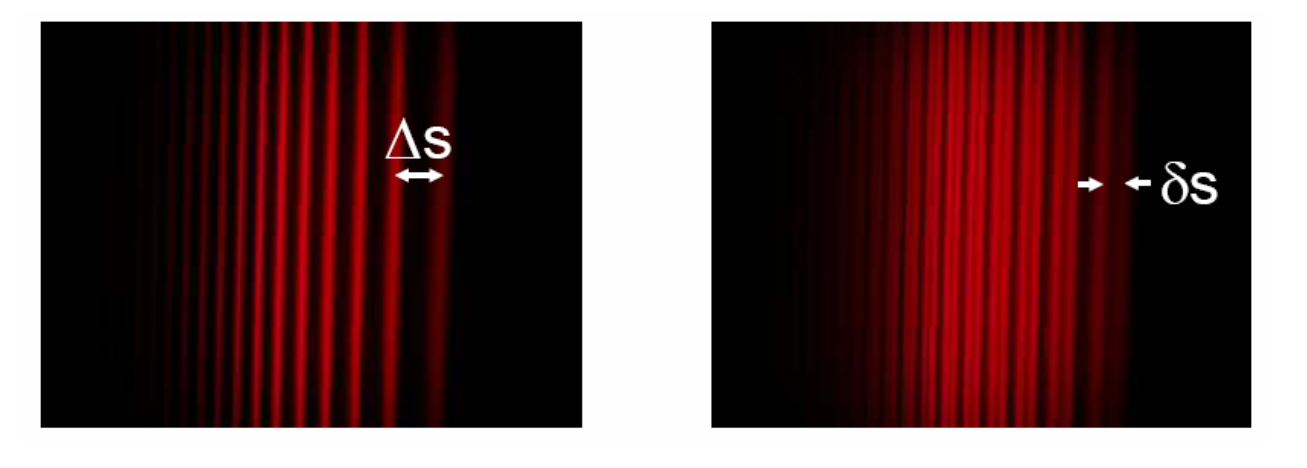
\includegraphics[width=0.7\textwidth]{pics/bsp_foto.png}
  \caption{Beispielhafte Aufnahme des Interferenzmusters der Lummer-Gehcke Platte.
  Links ohne Magnetfeld und rechts mit eingeschlatem Magnetfeld\cite{anleitung27}.}
  \label{fig: bsp_foto}
\end{figure}
\FloatBarrier
Danach wird der Elektromagnet eingeschaltet und das Magnetfeld so eingestellt das eine Aufspaltung der
Spektrallinen erkennbar ist (vgl. Abb. \ref{fig: bsp_foto}). Da beim normalen Zeemaneffekt, der Lande-Faktor konstant ist, lassen sich keine
Übergange mit $\Delta m$ beobachten, denn dort ist $\Delta E$. Deshlab wird bei rotem Licht nur
der $\sigma$ Übergang untersucht.


Abschließend soll noch blaues Licht $\lambda=\SI{480.0}{\nm}$, welches durch den Übergang $^3S_1\leftrightarrow ^3\!\!P_1$ emitiert wird,
analysiert werden \cite{anleitung27}. Ebenso wie beim roten Licht, muss zu beginn die Kamera justiert werden.
Danach wird ein Bild von dem Interferenzmuster ohne Magnetfeld gemacht. Wie in der Theorie besprochen ist der
Lande-Faktor für den anomalen Zemman-Effekt nicht mehr für jeden Zustand konstant. Auf Grund dessen muss hier der Polarisationfilter
so eingestellt werden, dass entweder nur der $\sigma$ oder $\pi$ Übergang beobachtbar ist. Nach einstellen des Magnetfeldes
und einstellen des Polarisationsfilter wird ein Bild von dem aufgespalteten Interferenzmuster geschossen. Die Durchführung wird jeweils für
einmal für den $\sigma$ Übergang und einmal für den $\pi$ Übergang vollzogen.


\subsection{Versuchsvorbereitung}
